\begin{figure}[htbp]
    \centering
    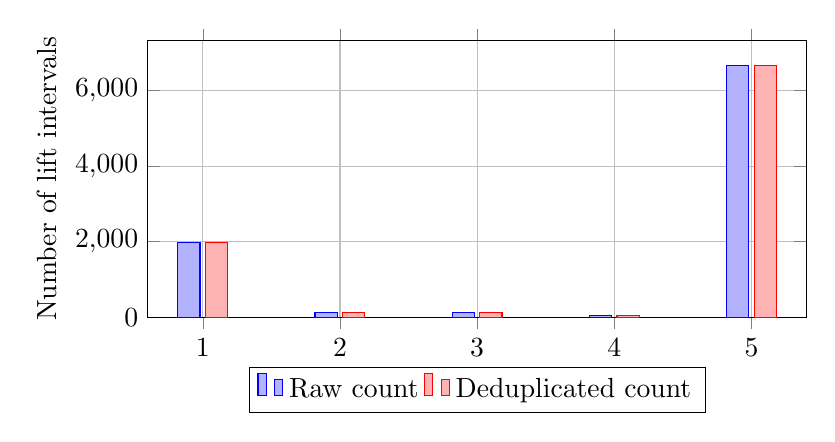
\begin{tikzpicture}
    \begin{axis}[
        width=0.82\linewidth,
        height=0.42\linewidth,
        ybar,
        bar width=8pt,
        xlabel={Movement type},
        ylabel={Number of lift intervals},
        symbolic x coords={1,2,3,4,5},
        xtick=data,
        ymin=0,
        legend style={at={(0.5,-0.18)}, anchor=north, legend columns=2},
        grid=major
    ]
        \addplot coordinates {
(1,1983)
(2,122)
(3,133)
(4,39)
(5,6658)
        };
        \addplot coordinates {
(1,1983)
(2,122)
(3,133)
(4,39)
(5,6658)
        };
        \legend{Raw count, Deduplicated count}
    \end{axis}
    \end{tikzpicture}
    \caption{Distribution of movement types before and after duplicate lift entries were removed.}
    \label{fig:movementtype-distribution}
\end{figure}
